\documentclass[final,hyperref={pdfpagelabels=false,unicode}]{beamer}
\usepackage{grffile}
\mode<presentation>{\usetheme{IAMS1}}
\usepackage[english]{babel}
\usepackage[latin1]{inputenc}
\usepackage{amsmath,amsthm, amssymb, latexsym}
%\usepackage{CJK}
%\usepackage{CJKutf8}

% \AtBeginDocument{%
%   \begin{CJK}{UTF8}{}}
% \AtEndDocument{%
%   \end{CJK}}

\boldmath
\usepackage[orientation=portrait,size=a0,scale=1.4,debug]{beamerposter}
% change list indention level
% \setdefaultleftmargin{3em}{}{}{}{}{}

%\usepackage{snapshot} % will write a .dep file with all dependencies, allows for easy bundling

\usepackage{array,booktabs,tabularx}
\newcolumntype{Z}{>{\centering\arraybackslash}X} % centered tabularx columns
\newcommand{\pphantom}{\textcolor{ta3aluminium}} % phantom introduces a vertical space in p formatted table columns??!!

\listfiles

%%%%%%%%%%%%%%%%%%%%%%%%%%%%%%%%%%%%%%%%%%%%%%%%%%%%%%%%%%%%%%%%%%%%%%%%%%%%%%%%%%%%%%
%% \graphicspath{{figures/}}



%\CJKfamily{bsmi}


% \author{Tsung-Han Wu (吳宗翰)}
% \author{Yan-Long Peng (彭彥龍)}
% \author{Sheng-Hui Lu (呂聖輝)}
% \author{Wang-Yau Cheng (鄭王曜)}
 
\title{\huge Ultra narrow dark resonance in high temperature caesium cell with mode-locked laser and buffer gas}
\author{G. Imreh, T-H. Wu, C-M. Wu, T-L. Yang, W-Y. Cheng}
\institute[IAMS, Academia Sinica]{Institute of Atomic and Molecular Sciences, Academia Sinica, Taiwan}
\date{\today}

%%%%%%%%%%%%%%%%%%%%%%%%%%%%%%%%%%%%%%%%%%%%%%%%%%%%%%%%%%%%%%%%%%%%%%%%%%%%%%%%%%%%%%
\newlength{\columnheight}
\setlength{\columnheight}{105cm}


%%%%%%%%%%%%%%%%%%%%%%%%%%%%%%%%%%%%%%%%%%%%%%%%%%%%%%%%%%%%%%%%%%%%%%%%%%%%%%%%%%%%%%
\begin{document}
\begin{frame}

  \begin{columns}
    % Left column
    \begin{column}{.49\textwidth}
      \begin{beamercolorbox}[center,wd=\textwidth]{postercolumn}
        \begin{minipage}[T]{.95\textwidth}
          % Parbox : to pull everything up to the top of the page, there might be better way than this
          \parbox[t][\columnheight]{\textwidth}{

            % Overview of our ideas
            \begin{block}{The coherent population trapping clock}
  \begin{itemize}
  \item The microwave frequency standard is cumbersome to link to the optical frequency range
  \item Coherent population trapping (CPT) or dark resonance is able to produce robust, narrow linewidth transitions, that can bridge the gap between microwave and optical freqencies
  \item In our scheme we further reduce the linewidth and eliminate light and pressure shifts of previous methods by:
    \begin{itemize}
    \item Mode-locked laser (short interaction time, high peak intensity)
    \item Using cesium (advantageous energy levels)
    \item High pressure buffer gas (pressure induced narrowing)
    \end{itemize}
  \item Potentials
    \begin{itemize}
    \item Frequency reference over a wide optical bandwith
    \item Frequency reference over large distances due to high peak power
    \item Compact, robust, all-optical system
    \end{itemize}
  \end{itemize}
\end{block}


            \vfill

            % Experimental setup
            \begin{block}{Experimental setup}
  \begin{figure}
    \begin{center}
      \includegraphics[width=.9\linewidth]{figures/experiment_big}
    \end{center}
    \label{Schematic of the experimental setup}
  \end{figure}
  $W$: output wedge, $BS$: beam splitter, $CTSDL$: cesium two-photon stabilized diode laser, $DG$: diffraction grating, $SLM$: spatial light modulator, $AOM$ acousto-optic modulator, $C$: mechanical chopper, $PMT$: photo-multiplier tube
  \begin{itemize}
  \item The repetition rate $f_{rep}$ is near integer fraction of the ground-state splitting (e.g. 1/100 $\approx$ 92 MHz )
  \item Repetition rate locked to 5th harmonic of synthetizer (that has 10~mHz stability)
  \item SLM band pass filter bandwith of $\approx$ 0.6 nm ($\approx$ 1 ps pulse length)
  \item Chopping frequency 500-1000 Hz
  \item Time-average input intensity 140$\mu$W with $<$1$\mu$W stability 
  \end{itemize}
\end{block}


            \vfill

            % Theoretical calculations
            \begin{block}{Theoretical considerations}
  \begin{itemize}
  \item Simulation uses simplified, 4-level system
  \item Build-up time of the order of 1 ms
  \item No need for frequency offset locking: mode-locked laser centre frequency drift does not affect CPT signal
  \item Small light shift compared to CW case
  \end{itemize}
  % %% Figures
  % \begin{figure}
  %   \includegraphics[width=0.5\textwidth]{}
  % \end{figure}
\end{block}


          }
        \end{minipage}
      \end{beamercolorbox}
    \end{column}
    % Right column
    \begin{column}{.49\textwidth}
      \begin{beamercolorbox}[center,wd=\textwidth]{postercolumn}
        \begin{minipage}[T]{.95\textwidth}
          % Parbox : to pull everything up to the top of the page, there might be better way than this
          \parbox[t][\columnheight]{\textwidth}{

            % Background
            \begin{block}{Atomic energy levels}
  \begin{itemize}
  \item A mode-locked laser excites the cesium atoms:
    \begin{itemize}
    \item Spectrum is a series of lines separated by the repetition rate
    \item Wide bandwith, can cover a large number of energy levels
    \end{itemize}
  \end{itemize}
  \begin{columns}
    \begin{column}{0.49\textwidth}
      \begin{figure}
        \begin{center}
          \includegraphics[width=.85\textwidth]{figures/energylevels}
        \end{center}
      \end{figure}
      \begin{itemize}
      \item Coherent population trapping in the hyperfine ground states
      \item Excited state is on the D2 transition
      \item Input light is band-pass filtered to reduce scattered background
      \end{itemize}
    \end{column}
    \begin{column}{0.49\textwidth}
      \begin{figure}
        \begin{center}
          
\includegraphics[width=.6\textwidth]{figures/modelockresonance}
        \end{center}
      \end{figure}
      \begin{itemize}
      \item The mode-locked laser have multiple resonance conditions between the excited state ($E$) and the two ground states ($G_1$ and $G_2$)
      \item Interaction is tuned by the repetition rate 
      \end{itemize}
    \end{column}
  \end{columns}
\end{block}

            \vfill

            % Experimental results
            \begin{block}{Experimental results}
  Put pretty pictures here
\end{block}

            \vfill

            % Future work, etc...
            \begin{block}{Outlook - the optical ladder}
  Our group developed compact frequency standards for two differen Cs transitions. Combine this with a frequency comb to get an optical ladder.
  \begin{columns}
    \begin{column}{0.49\textwidth}
     \begin{itemize}
     \item 822 nm reference locks the repetition rate
     \item 884 nm reference lock the absolute frequency
     \item CPT transition provides monitoring of the repetition rate, connecting the microwave and optical regime
     \end{itemize}
    \end{column}
    \begin{column}{0.49\textwidth}
      \begin{figure}
        \begin{center}
          \includegraphics[width=1.0\textwidth]{figures/vernier}
        \end{center}
      \end{figure}
    \end{column}
  \end{columns}
  This scheme removes the need of a highly stable synthetizer, which is an obstacle to a compact and robust design.
\end{block}

          }
        \end{minipage}
      \end{beamercolorbox}
    \end{column}
  \end{columns}
%  \vskip1ex
\end{frame}
\end{document}


%%%%%%%%%%%%%%%%%%%%%%%%%%%%%%%%%%%%%%%%%%%%%%%%%%%%%%%%%%%%%%%%%%%%%%%%%%%%%%%%%%%%%%%%%%%%%%%%%%%%
%%% Local Variables: 
%%% mode: latex
%%% TeX-PDF-mode: t
%%% End:
